\begin{wrapfigure}[0]{r}[9pt]{0cm}
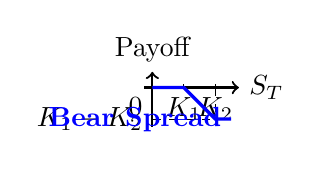
\begin{tikzpicture}[scale=1]
    % --- 定义坐标和参数 ---
    \def\Kone{0.4}       % 行权价 K1
    \def\Ktwo{0.8}       % 行权价 K2 (K2 > K1)
    \def\maxST{1}      % S_T 的最大显示范围

    % [修改处] 引入一个新的变量来控制最大损失线的视觉位置
    % 原来的数学计算值是 -(\Ktwo - \Kone) = -0.4
    % 现在手动设置一个更靠上的位置，比如 -0.25
    \def\visualLossLevel{-0.4}

    % --- 绘制坐标轴 ---
    % Y 轴 (Payoff) - 根据新的视觉水平调整绘制范围
    \draw[->, thick] (0, \visualLossLevel - 0.1) -- (0, 0.2) node[above] {Payoff};
    % X 轴 (S_T)
    \draw[->, thick] (-0.1, 0) -- (\maxST + 0.1, 0) node[right] {$S_T$};

    % --- 绘制辅助线和标签 ---
    % 标记原点
    \node[below left] at (0, 0) {0};

    % 在 X 轴上标记 K1
    \draw (\Kone, 0) node[below] {$K_1$} -- (\Kone, 0.05);

    % 在 X 轴上标记 K2
    \draw (\Ktwo, 0) node[below] {$K_2$} -- (\Ktwo, 0.05);

    % --- [修改处] 在 Y 轴上标记最大损失 ---
    % 使用新的视觉坐标 \visualLossLevel 来绘制刻度线和放置标签
    % 标签文字保持数学含义 $K_1 - K_2$ 不变
    \draw (0, \visualLossLevel) node[left] {$K_1 - K_2$} -- (0.05, \visualLossLevel);

    % 绘制辅助虚线
    % 垂直线的终点使用新的视觉坐标
    \draw[dashed, thin] (\Ktwo, 0) -- (\Ktwo, \visualLossLevel);
    % 水平线使用新的视觉坐标
    \draw[dashed, thin] (0, \visualLossLevel) -- (\Ktwo, \visualLossLevel);


    % --- 绘制熊市价差收益曲线 (蓝色粗线) ---
    % [修改处] 将曲线转折点和终点的 Y 坐标改为新的视觉坐标 \visualLossLevel
    % 路径: (0,0) -> (K1, 0) -> (K2, \visualLossLevel) -> (maxST, \visualLossLevel)
    \draw[blue, very thick] (0, 0) -- (\Kone, 0) -- (\Ktwo, \visualLossLevel) -- (\maxST, \visualLossLevel);

    % --- 添加标题标签 ---
    % [修改处] 标题的位置也跟随调整到新的视觉水平
    \node[blue, anchor=south east, font=\bfseries, yshift= -8pt] at (\maxST, \visualLossLevel) {Bear Spread};

\end{tikzpicture}
\end{wrapfigure}